\begin{figure*}[t]
	\centering
	\begin{minipage}{0.3\textwidth}
		\centering
		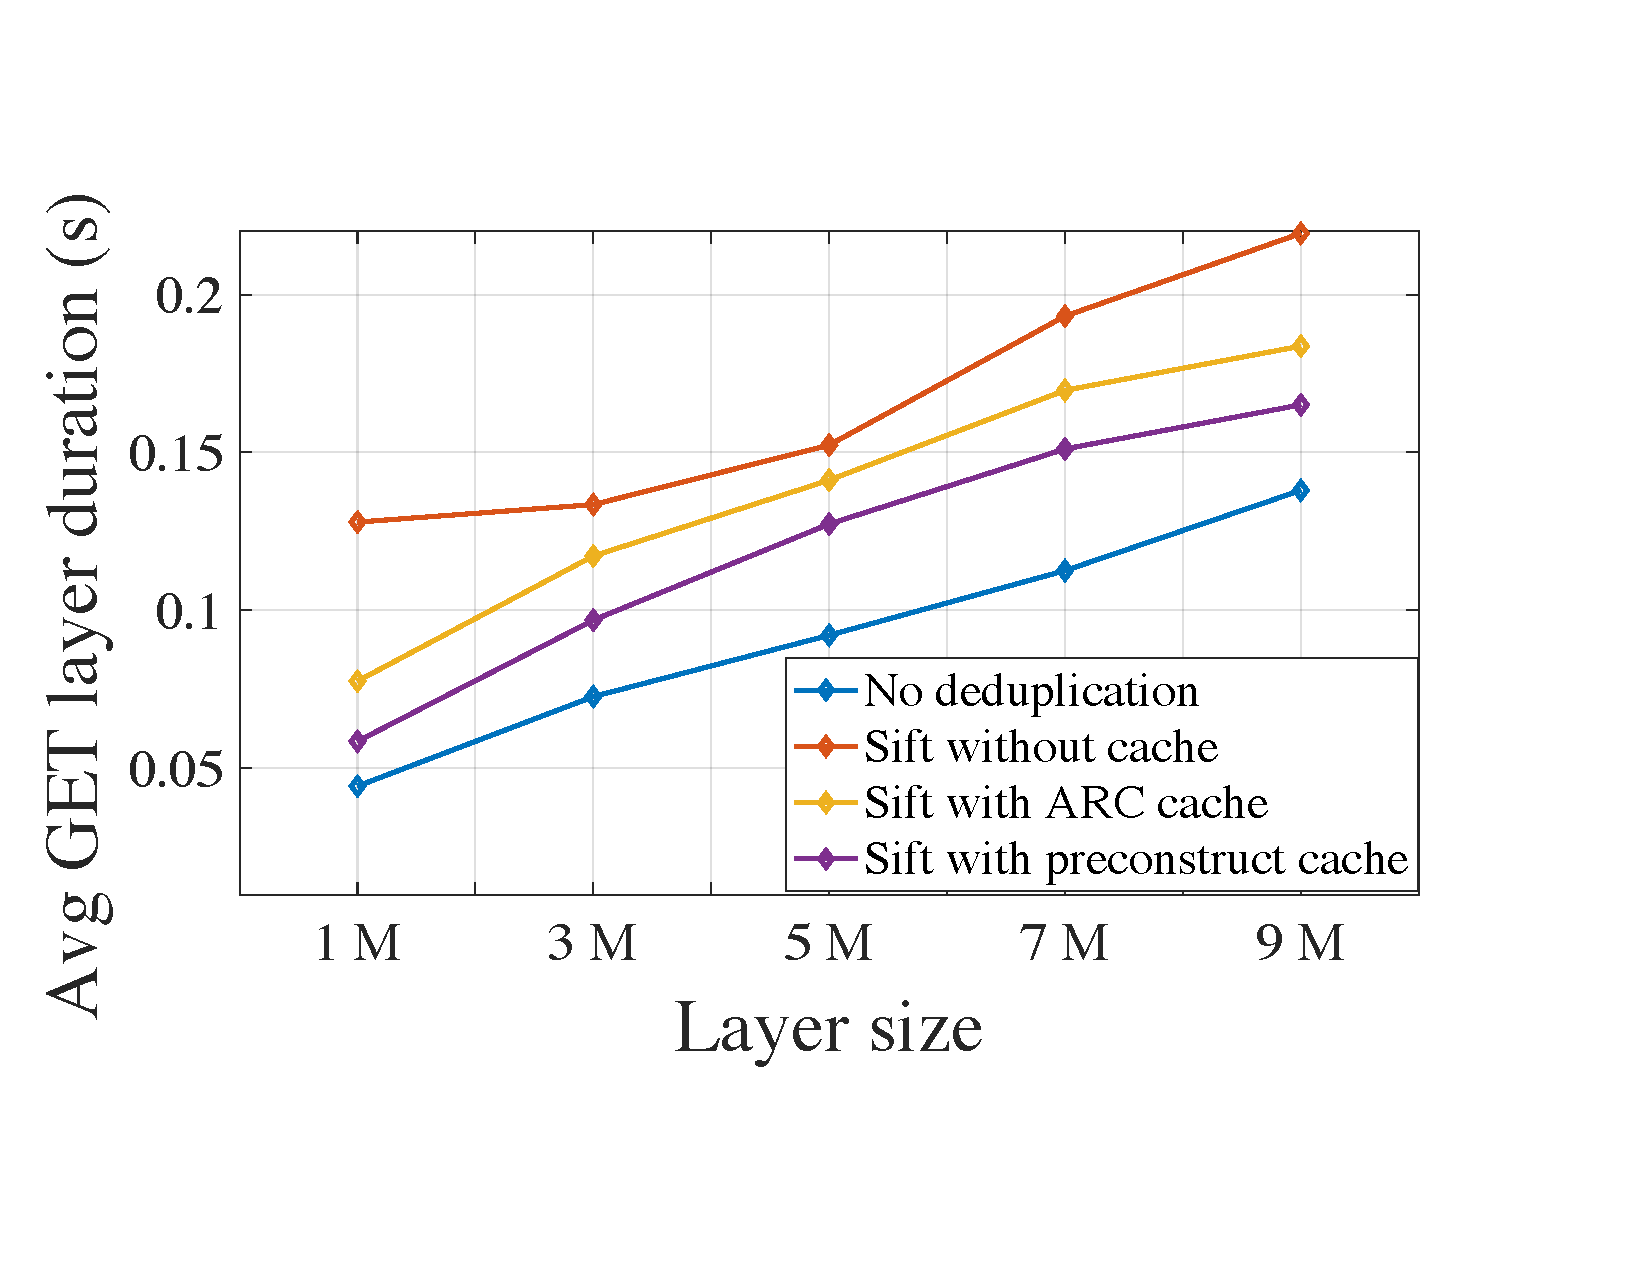
\includegraphics[width=0.9\textwidth]{graphs/1nodegetlayerlatency.pdf}
		\caption{GET layer latency.\todo{add grid in background to match the other figures}}% across different schemes.}
		\label{fig:eval-1nodegetlayerlatency}
	\end{minipage}%
	\begin{minipage}{0.3\textwidth}
		\centering
		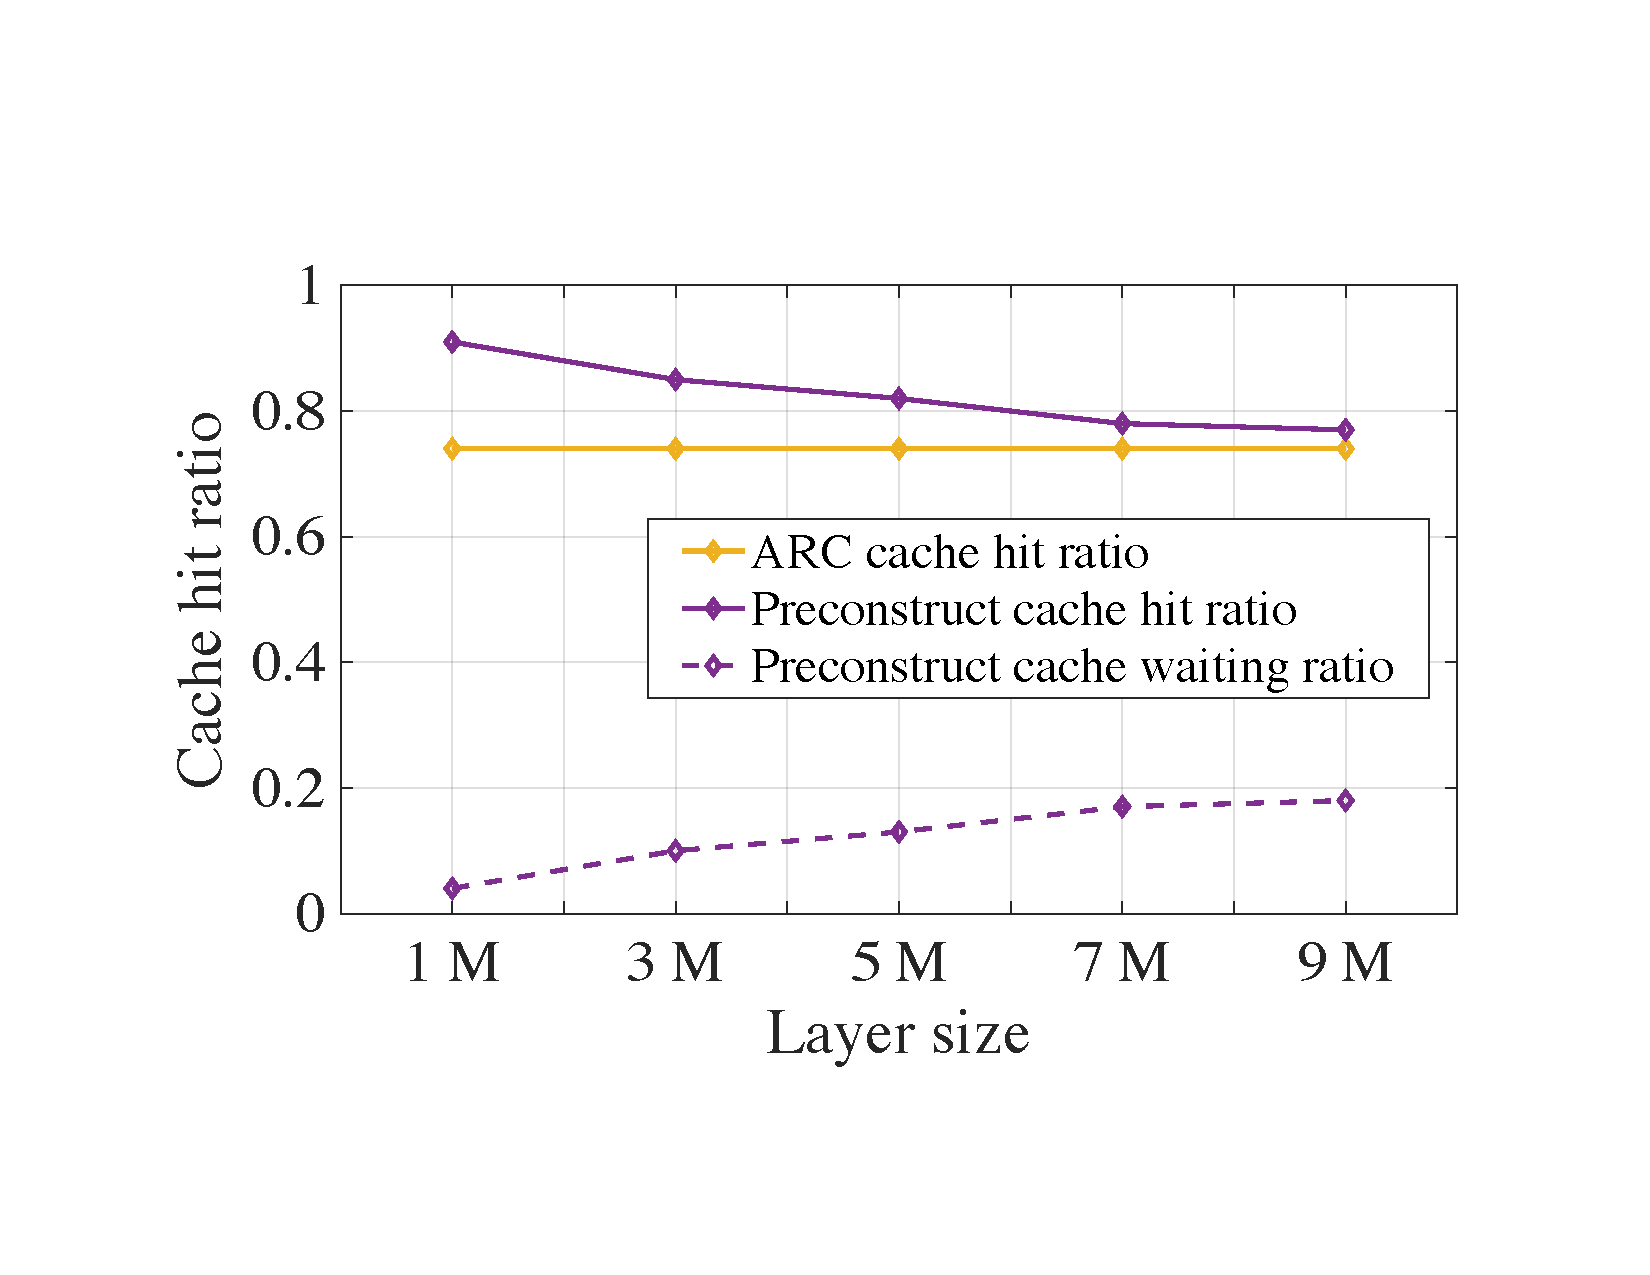
\includegraphics[width=0.9\textwidth]{graphs/cachehitratio.pdf}
		\caption{Cache hit ratio.}% of LRU cache and preconstruct cache.}
		\label{fig:eval-cachehitratios}
	\end{minipage}%
	\begin{minipage}{0.3\textwidth}
	\centering
	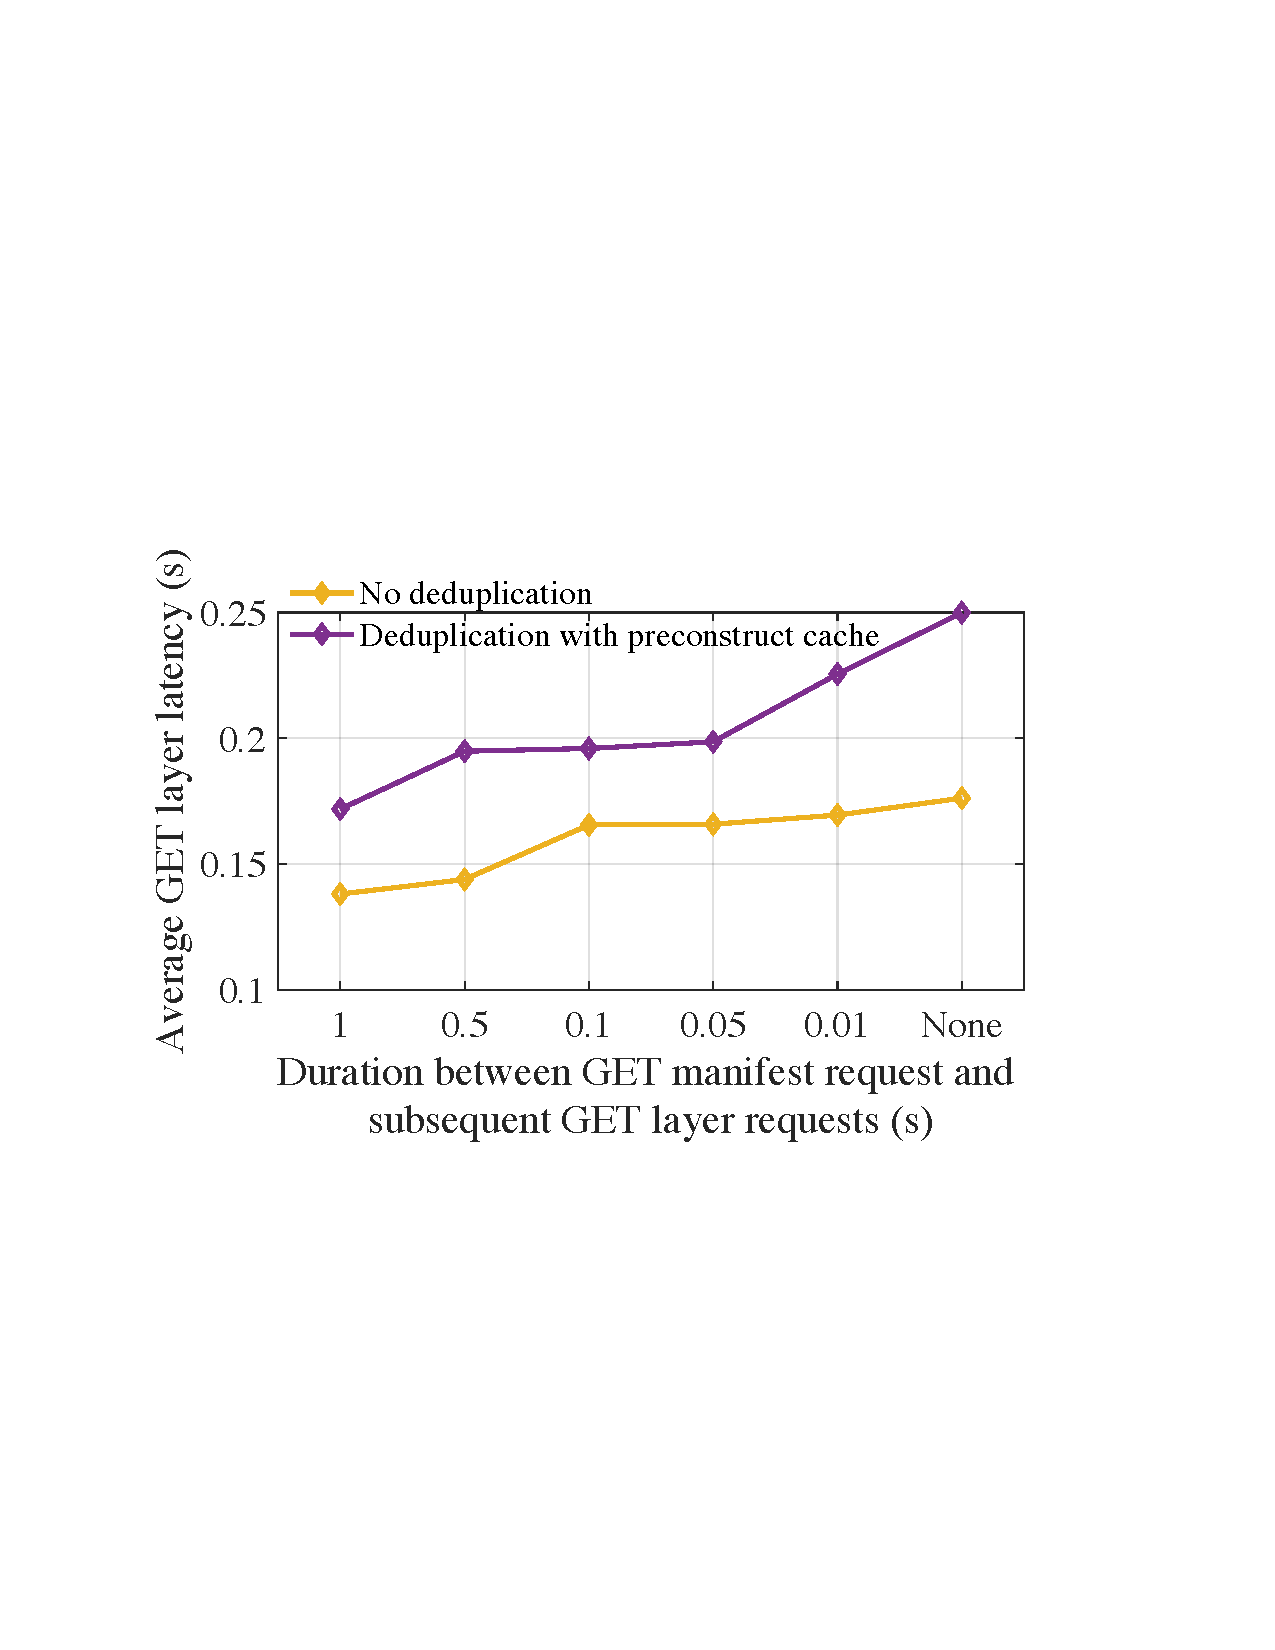
\includegraphics[width=0.9\textwidth]{graphs/durationML.pdf}
	\caption{The impact of durationML.}
	\label{fig:eval-durationML}
   \end{minipage}

\end{figure*}


\begin{figure*}[t]
	\centering
	\begin{minipage}{0.3\textwidth}
		\centering
		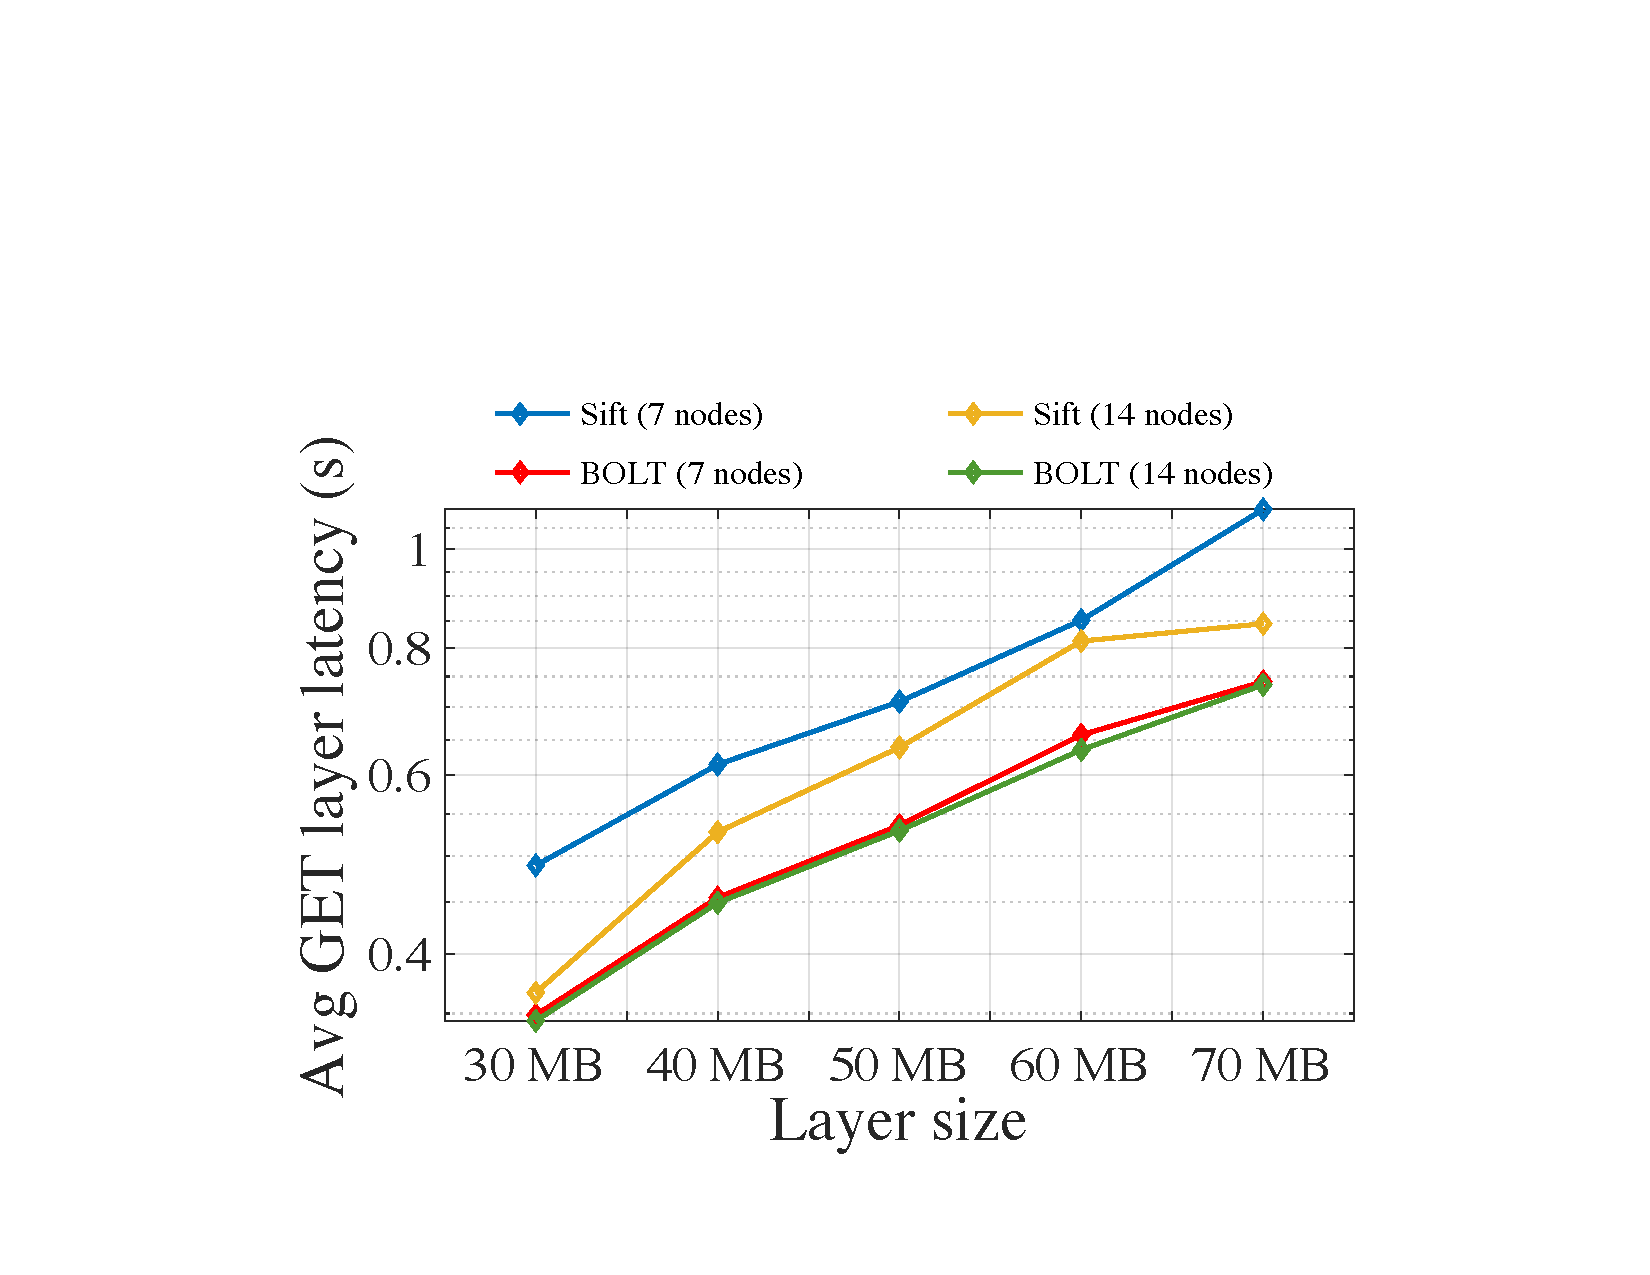
\includegraphics[width=0.9\textwidth]{graphs/clusterscale.pdf}
		\caption{GET layer latency with different cluster size. \Subil{the blue line is peeking out of the box.} \todo{change object storage to BOLT in figure}}
		\label{fig:eval-clusterscale}
	\end{minipage}%
	\hspace{1mm}
	\begin{minipage}{0.3\textwidth}
	\centering
	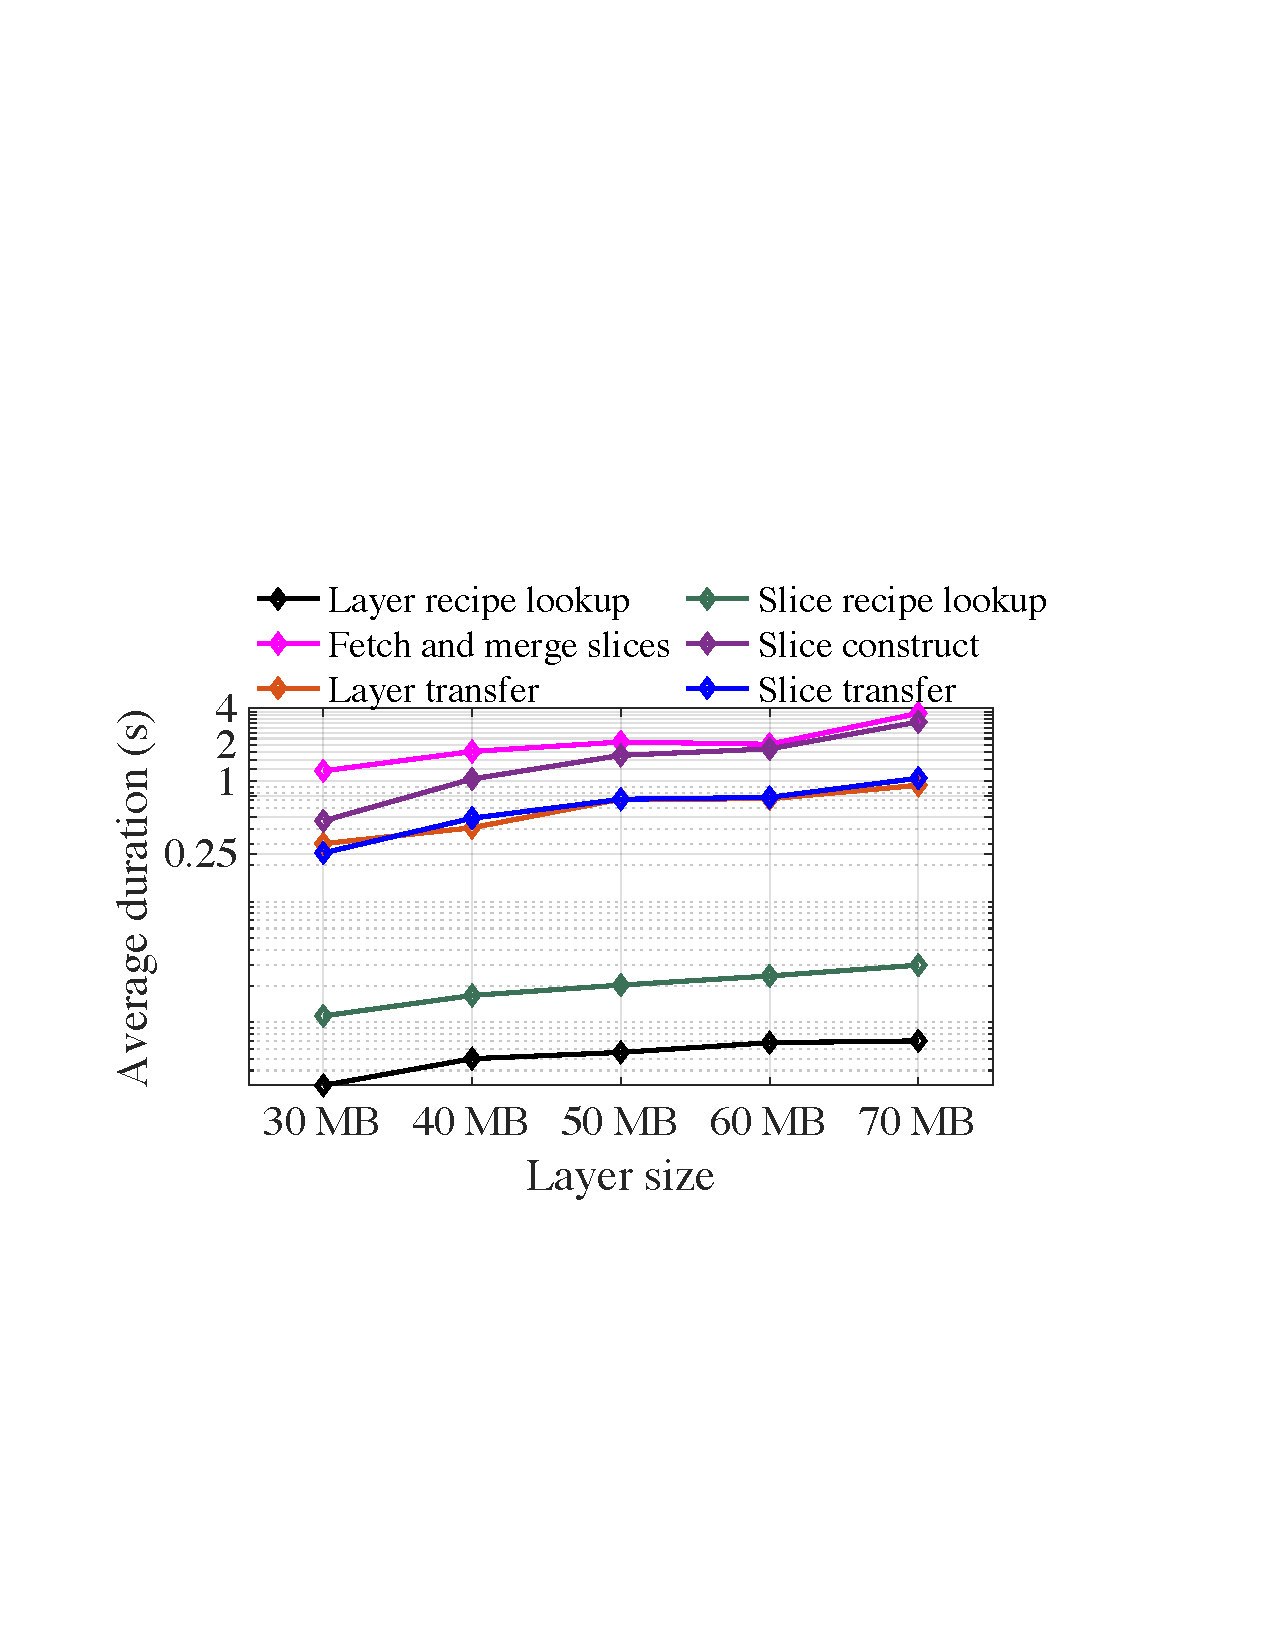
\includegraphics[width=0.9\textwidth]{graphs/restoringbreakdown.pdf}
	\caption{Restoring latency breakdown. \Subil{maybe change 'fetch and merge slices' to 'layer construction duration' to keep consistency with the text}}
	\label{fig:eval-restoringbreakdown}
	\end{minipage}
	\hspace{1mm}
	\begin{minipage}{0.3\textwidth}
		\centering
		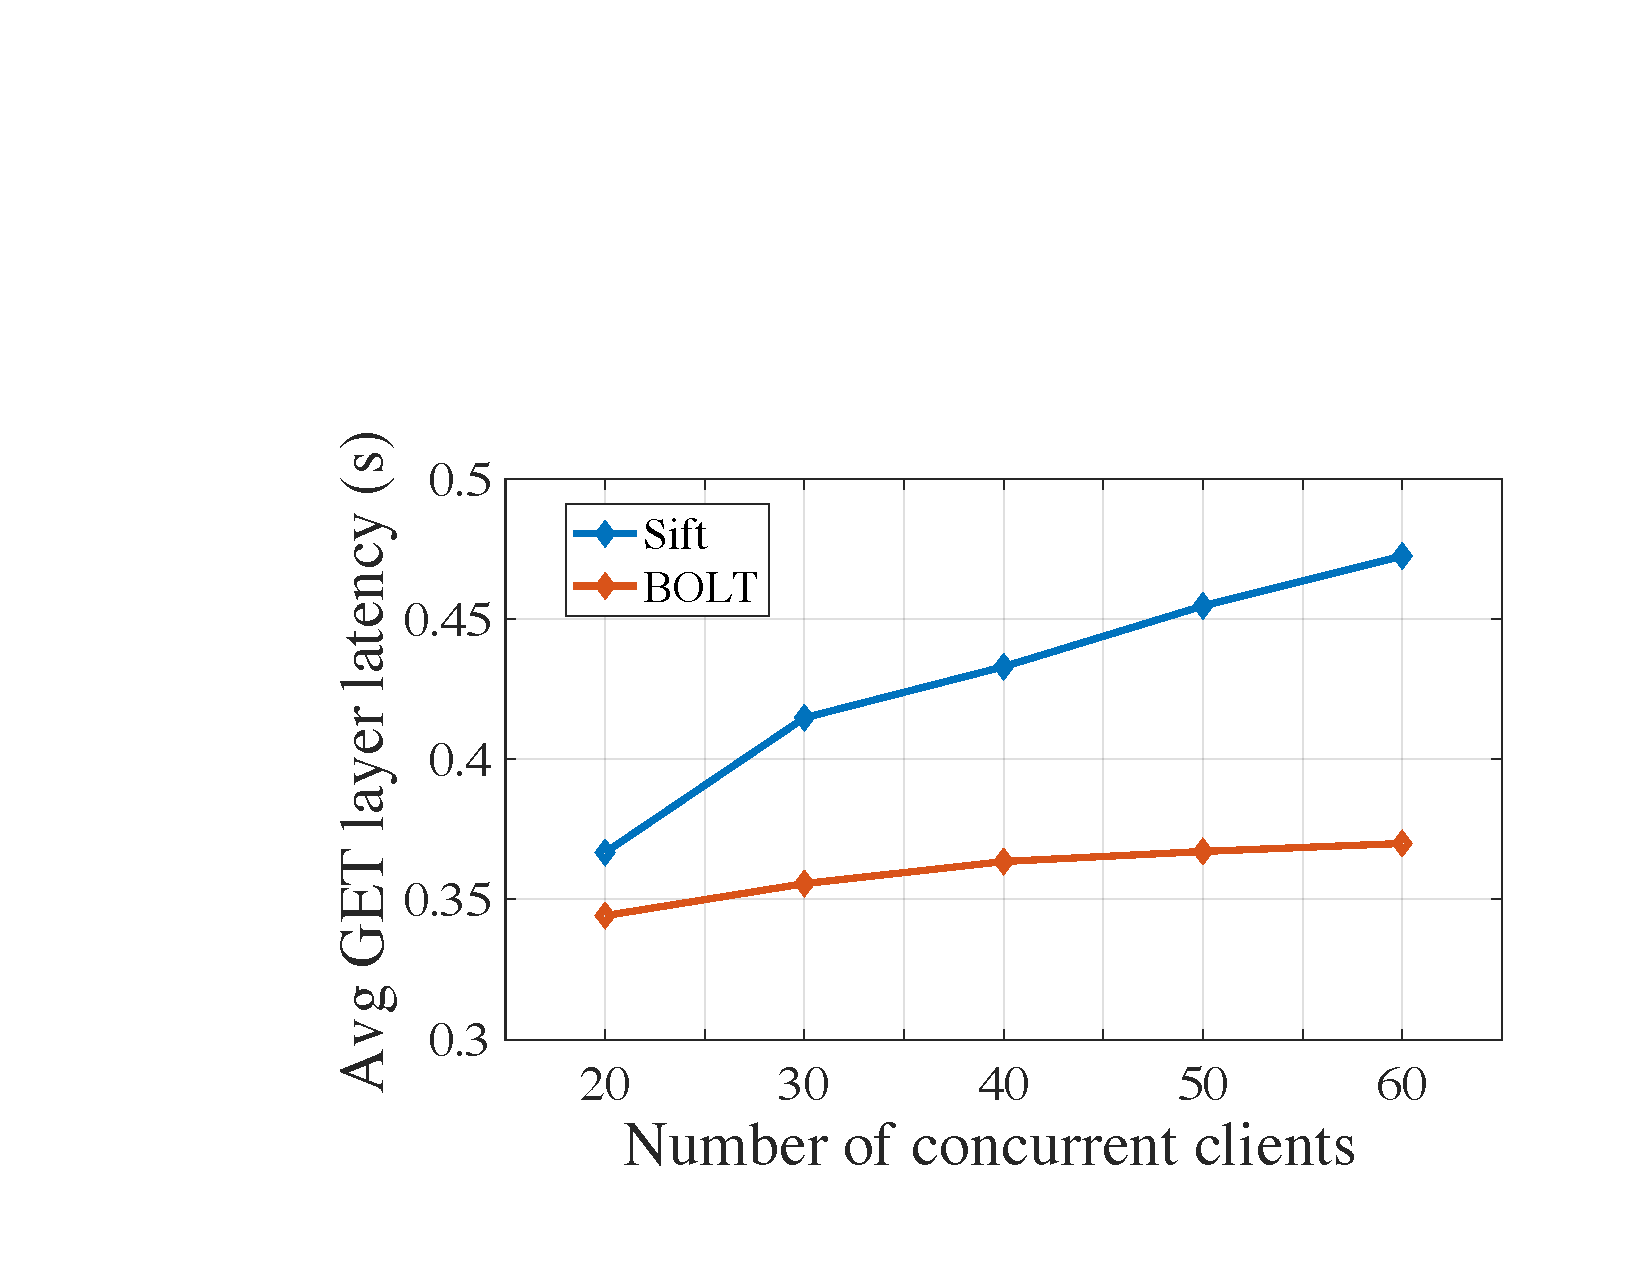
\includegraphics[width=0.9\textwidth]{graphs/clientscale.pdf}
		\caption{GET layer latency with different client concurrency.}
		\label{fig:eval-clientscale}
	\end{minipage}%	
\end{figure*}

\begin{figure}[t]
	\centering
	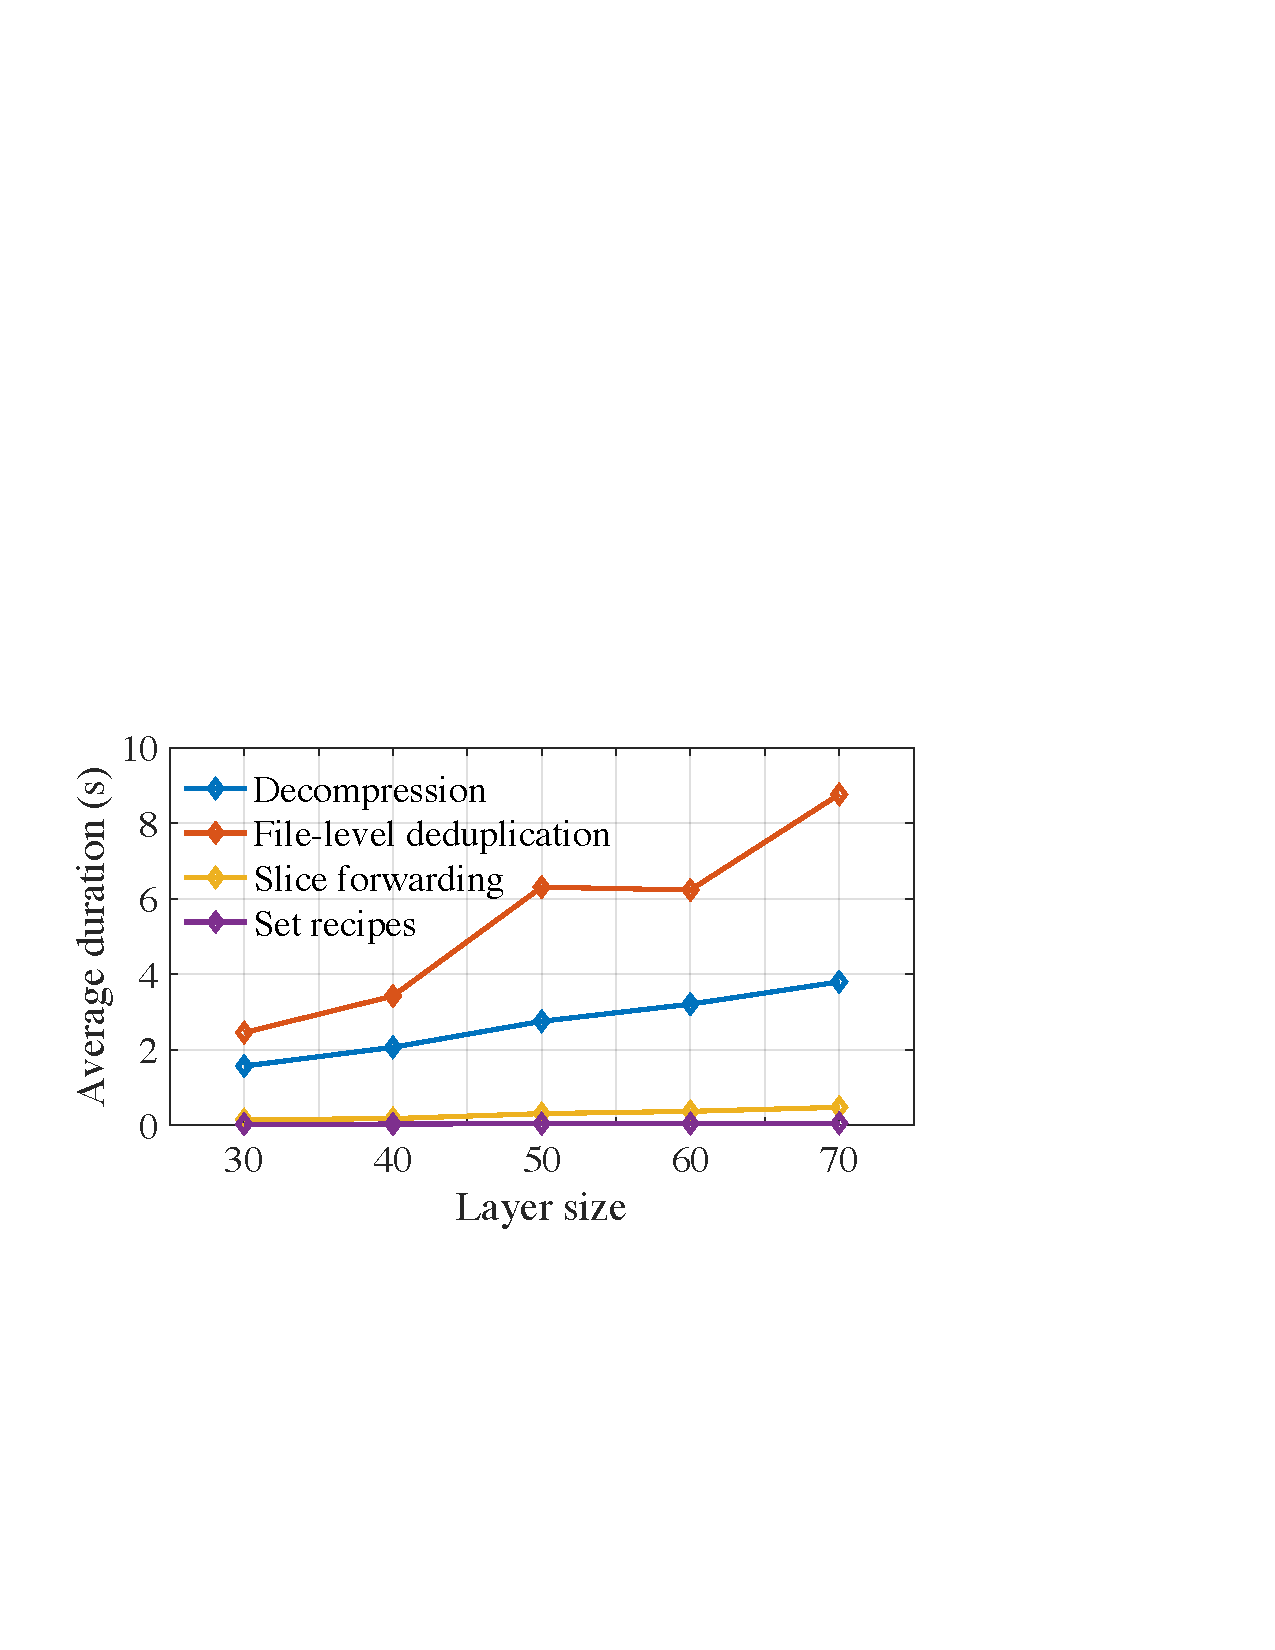
\includegraphics[width=0.3\textwidth]{graphs/dedupbreakdown.pdf}
	\caption{Deduplication latency breakdown.}
	%	\vspace{-3pt}
	\label{fig:eval-dedupbreakdown}
	
\end{figure}